\documentclass[11pt,]{article}
\usepackage{lmodern}
\usepackage{amssymb,amsmath}
\usepackage{ifxetex,ifluatex}
\usepackage{fixltx2e} % provides \textsubscript
\ifnum 0\ifxetex 1\fi\ifluatex 1\fi=0 % if pdftex
  \usepackage[T1]{fontenc}
  \usepackage[utf8]{inputenc}
\else % if luatex or xelatex
  \ifxetex
    \usepackage{mathspec}
  \else
    \usepackage{fontspec}
  \fi
  \defaultfontfeatures{Ligatures=TeX,Scale=MatchLowercase}
\fi
% use upquote if available, for straight quotes in verbatim environments
\IfFileExists{upquote.sty}{\usepackage{upquote}}{}
% use microtype if available
\IfFileExists{microtype.sty}{%
\usepackage{microtype}
\UseMicrotypeSet[protrusion]{basicmath} % disable protrusion for tt fonts
}{}
\usepackage[margin = 1.5in]{geometry}
\usepackage{hyperref}
\PassOptionsToPackage{usenames,dvipsnames}{color} % color is loaded by hyperref
\hypersetup{unicode=true,
            pdftitle={Optimization},
            pdfauthor={Abhinav Anand, IIMB},
            colorlinks=true,
            linkcolor=blue,
            citecolor=magenta,
            urlcolor=red,
            breaklinks=true}
\urlstyle{same}  % don't use monospace font for urls
\usepackage{color}
\usepackage{fancyvrb}
\newcommand{\VerbBar}{|}
\newcommand{\VERB}{\Verb[commandchars=\\\{\}]}
\DefineVerbatimEnvironment{Highlighting}{Verbatim}{commandchars=\\\{\}}
% Add ',fontsize=\small' for more characters per line
\usepackage{framed}
\definecolor{shadecolor}{RGB}{248,248,248}
\newenvironment{Shaded}{\begin{snugshade}}{\end{snugshade}}
\newcommand{\KeywordTok}[1]{\textcolor[rgb]{0.13,0.29,0.53}{\textbf{#1}}}
\newcommand{\DataTypeTok}[1]{\textcolor[rgb]{0.13,0.29,0.53}{#1}}
\newcommand{\DecValTok}[1]{\textcolor[rgb]{0.00,0.00,0.81}{#1}}
\newcommand{\BaseNTok}[1]{\textcolor[rgb]{0.00,0.00,0.81}{#1}}
\newcommand{\FloatTok}[1]{\textcolor[rgb]{0.00,0.00,0.81}{#1}}
\newcommand{\ConstantTok}[1]{\textcolor[rgb]{0.00,0.00,0.00}{#1}}
\newcommand{\CharTok}[1]{\textcolor[rgb]{0.31,0.60,0.02}{#1}}
\newcommand{\SpecialCharTok}[1]{\textcolor[rgb]{0.00,0.00,0.00}{#1}}
\newcommand{\StringTok}[1]{\textcolor[rgb]{0.31,0.60,0.02}{#1}}
\newcommand{\VerbatimStringTok}[1]{\textcolor[rgb]{0.31,0.60,0.02}{#1}}
\newcommand{\SpecialStringTok}[1]{\textcolor[rgb]{0.31,0.60,0.02}{#1}}
\newcommand{\ImportTok}[1]{#1}
\newcommand{\CommentTok}[1]{\textcolor[rgb]{0.56,0.35,0.01}{\textit{#1}}}
\newcommand{\DocumentationTok}[1]{\textcolor[rgb]{0.56,0.35,0.01}{\textbf{\textit{#1}}}}
\newcommand{\AnnotationTok}[1]{\textcolor[rgb]{0.56,0.35,0.01}{\textbf{\textit{#1}}}}
\newcommand{\CommentVarTok}[1]{\textcolor[rgb]{0.56,0.35,0.01}{\textbf{\textit{#1}}}}
\newcommand{\OtherTok}[1]{\textcolor[rgb]{0.56,0.35,0.01}{#1}}
\newcommand{\FunctionTok}[1]{\textcolor[rgb]{0.00,0.00,0.00}{#1}}
\newcommand{\VariableTok}[1]{\textcolor[rgb]{0.00,0.00,0.00}{#1}}
\newcommand{\ControlFlowTok}[1]{\textcolor[rgb]{0.13,0.29,0.53}{\textbf{#1}}}
\newcommand{\OperatorTok}[1]{\textcolor[rgb]{0.81,0.36,0.00}{\textbf{#1}}}
\newcommand{\BuiltInTok}[1]{#1}
\newcommand{\ExtensionTok}[1]{#1}
\newcommand{\PreprocessorTok}[1]{\textcolor[rgb]{0.56,0.35,0.01}{\textit{#1}}}
\newcommand{\AttributeTok}[1]{\textcolor[rgb]{0.77,0.63,0.00}{#1}}
\newcommand{\RegionMarkerTok}[1]{#1}
\newcommand{\InformationTok}[1]{\textcolor[rgb]{0.56,0.35,0.01}{\textbf{\textit{#1}}}}
\newcommand{\WarningTok}[1]{\textcolor[rgb]{0.56,0.35,0.01}{\textbf{\textit{#1}}}}
\newcommand{\AlertTok}[1]{\textcolor[rgb]{0.94,0.16,0.16}{#1}}
\newcommand{\ErrorTok}[1]{\textcolor[rgb]{0.64,0.00,0.00}{\textbf{#1}}}
\newcommand{\NormalTok}[1]{#1}
\usepackage{graphicx,grffile}
\makeatletter
\def\maxwidth{\ifdim\Gin@nat@width>\linewidth\linewidth\else\Gin@nat@width\fi}
\def\maxheight{\ifdim\Gin@nat@height>\textheight\textheight\else\Gin@nat@height\fi}
\makeatother
% Scale images if necessary, so that they will not overflow the page
% margins by default, and it is still possible to overwrite the defaults
% using explicit options in \includegraphics[width, height, ...]{}
\setkeys{Gin}{width=\maxwidth,height=\maxheight,keepaspectratio}
\IfFileExists{parskip.sty}{%
\usepackage{parskip}
}{% else
\setlength{\parindent}{0pt}
\setlength{\parskip}{6pt plus 2pt minus 1pt}
}
\setlength{\emergencystretch}{3em}  % prevent overfull lines
\providecommand{\tightlist}{%
  \setlength{\itemsep}{0pt}\setlength{\parskip}{0pt}}
\setcounter{secnumdepth}{0}
% Redefines (sub)paragraphs to behave more like sections
\ifx\paragraph\undefined\else
\let\oldparagraph\paragraph
\renewcommand{\paragraph}[1]{\oldparagraph{#1}\mbox{}}
\fi
\ifx\subparagraph\undefined\else
\let\oldsubparagraph\subparagraph
\renewcommand{\subparagraph}[1]{\oldsubparagraph{#1}\mbox{}}
\fi

%%% Use protect on footnotes to avoid problems with footnotes in titles
\let\rmarkdownfootnote\footnote%
\def\footnote{\protect\rmarkdownfootnote}

%%% Change title format to be more compact
\usepackage{titling}

% Create subtitle command for use in maketitle
\newcommand{\subtitle}[1]{
  \posttitle{
    \begin{center}\large#1\end{center}
    }
}

\setlength{\droptitle}{-2em}
  \title{Optimization}
  \pretitle{\vspace{\droptitle}\centering\huge}
  \posttitle{\par}
  \author{Abhinav Anand, IIMB}
  \preauthor{\centering\large\emph}
  \postauthor{\par}
  \predate{\centering\large\emph}
  \postdate{\par}
  \date{2018/06/11}

\linespread{1.25}
\usepackage{amsmath}

\begin{document}
\maketitle

\section{Background}\label{background}

Problems in finance and economics are often concerned with the behavior
of agents who are considered to be utility maximizers. Utility functions
are thought to be monotonic in their variables---more of a utility
enhancing variable is better than less---and are thought to obey
diminishing returns as the variables scale.\footnote{This utility
  function can assume a variety of forms. For example, if the `agent' is
  a firm, its utility is its profit function; if its a government, it
  could be some (aggregate) social welfare function etc.} Additionally,
real-life constraints ensure that variables are bounded. Hence
optimization of functions under constraints forms an important
discipline in the study of such subjects.

After linear optimization, quadratic optimization problems are the
simplest since they can be captured in \emph{quadratic forms} and can be
represented via symmetric matrices with special properties. A
distinguishing feature of quadratic optimization is the presence of
first and second order conditions that characterize the nature of the
extreme point.

\subsection{Quadratic Optimization}\label{quadratic-optimization}

In one dimension, \(x\in \mathbb{R}\) the simplest quadratic objective
functions can be \(f(x)=\{x^2, -x^2\}\) with the first attaining a
global minimum and the second a global maximum at \(x=0\).

\begin{Shaded}
\begin{Highlighting}[]
\NormalTok{x <-}\StringTok{ }\OperatorTok{-}\DecValTok{500}\OperatorTok{:}\DecValTok{500}
\NormalTok{y_}\DecValTok{1}\NormalTok{ <-}\StringTok{ }\NormalTok{x}\OperatorTok{^}\DecValTok{2}
\NormalTok{y_}\DecValTok{2}\NormalTok{ <-}\StringTok{ }\OperatorTok{-}\NormalTok{x}\OperatorTok{^}\DecValTok{2}
\NormalTok{data_l <-}\StringTok{ }\KeywordTok{cbind}\NormalTok{(x, y_}\DecValTok{1}\NormalTok{, y_}\DecValTok{2}\NormalTok{) }\OperatorTok\StringTok{ }
\StringTok{  }\NormalTok{dplyr}\OperatorTok{::}\KeywordTok{as_tibble}\NormalTok{() }\OperatorTok\StringTok{ }\CommentTok{#wide format}
\StringTok{  }\NormalTok{tidyr}\OperatorTok{::}\KeywordTok{gather}\NormalTok{(., }
\NormalTok{                y_}\DecValTok{1}\OperatorTok{:}\NormalTok{y_}\DecValTok{2}\NormalTok{, }
                \DataTypeTok{key =} \StringTok{'y'}\NormalTok{, }
                \DataTypeTok{value =} \StringTok{'f'}\NormalTok{) }\CommentTok{#long format}

\KeywordTok{ggplot}\NormalTok{(data_l, }\KeywordTok{aes}\NormalTok{(x, f, }\DataTypeTok{color =}\NormalTok{ y)) }\OperatorTok{+}
\StringTok{  }\KeywordTok{geom_line}\NormalTok{() }\OperatorTok{+}
\StringTok{  }\KeywordTok{geom_hline}\NormalTok{(}\DataTypeTok{yintercept =} \DecValTok{0}\NormalTok{) }\OperatorTok{+}
\StringTok{  }\KeywordTok{theme_minimal}\NormalTok{()}
\end{Highlighting}
\end{Shaded}

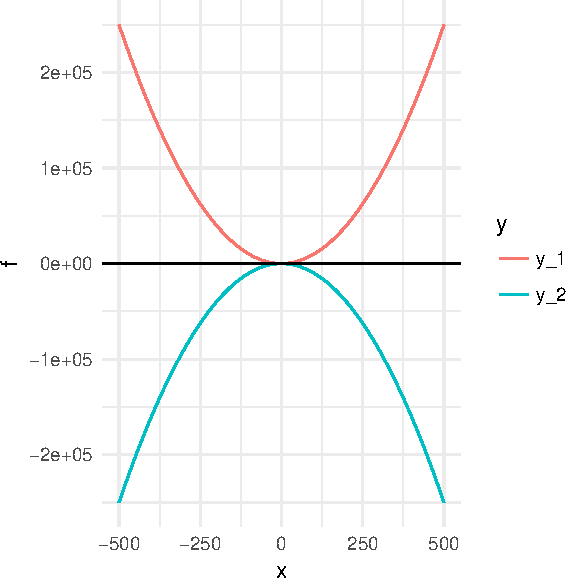
\includegraphics{Optimization_files/figure-latex/opt_dim_1-1.pdf}

\subsubsection{Quadratic Forms}\label{quadratic-forms}

For the case when \(x = (x_1, x_2) \in \mathbb{R}^2\), a general
quadratic form is the following: \[
Q(x) = a_{11}x_1^2 + a_{22}x_2^2 + 2a_{12}x_1x_2
\] which may be represented as a matrix: \[
Q(x) = [x_1 x_2]\begin{bmatrix}a_{11} & a_{12}\\ a_{12} & a_{22}\end{bmatrix}
\begin{bmatrix}x_1 \\ x_2\end{bmatrix}
\] Similarly, when \(x = (x_1, x_2, x_3) \in \mathbb{R}^3\), the form
becomes \[
Q(x) = [x_1 x_2 x_3]\begin{bmatrix}a_{11} & a_{12} & a_{13}\\ a_{12} & a_{22} & a_{23}\\
a_{13} & a_{23} & a_{33}\end{bmatrix} \begin{bmatrix}x_1 \\ x_2 \\ x_3\end{bmatrix}
\] and in general, when \(x = (x_1, \hdots, x_n) \in \mathbb{R}^n\): \[
Q(x) = [x_1 \hdots x_n]\begin{bmatrix}a_{11} & \hdots & a_{1n}\\ \vdots\\
a_{1n} & \hdots & a_{nn}\end{bmatrix} \begin{bmatrix}x_1\\ \vdots\\ x_n\end{bmatrix}
\] It's easy to see that \(Q(0) = 0\). If \(a>0, ax^2>0\) and we can
call the quadratic form ``positive definite''. Similarly, if
\(a<0, ax^2<0\) and we call the form ``negative definite''. This carries
over when \(x\in \mathbb{R}^2\), since \(Q(x_1, x_2) = x_1^2+x_2^2>0\)
(positive definite) and \(Q(x_1, x_2) = -x_1^2-x_2^2>0\) (negative
definite). Additionally for the case when
\(Q(x_1, x_2) = x_1^2-x_2^2>0\), the quadratic form is
\emph{indefinite}.

In general, symmetric matrices are called positive (semi)definite,
negative (semi)definite etc. according to the definiteness of the
expression \(Q(x) = x^{\top}Ax\).\footnote{Hence if
  \(\forall x\neq0\in \mathbb{R}^n, x^{\top}Ax\geq 0\) the form is
  positive semidefinite and so on.}

\section{Unconstrained Optimization}\label{unconstrained-optimization}

While it's clear what a maximum is in one dimension, what should be its
definition in two dimensions and beyond? The central idea remains the
same: \(x^*\) is the maximum if there is no other \(x\) in the domain of
\(f(x)\) such that \(f(x)\geq f(x^*)\). Note that this definition is
general and independent of the dimension of the underlying space from
where we pick \(x\). The only difference in dimensions one and beyond is
the structure of the domain; and while in one dimension it must take the
form \(x_L\leq x\leq x_H\), one needs such conditions for each component
when
\(x\in \mathbb{R}^n: x_{L1}\leq x_1\leq x_{H1}, \hdots, x_{Ln}\leq x_n\leq x_{Hn}\).
With this interpretation in mind, we are ready to formulate the
necessary and sufficient conditions for the optimal of an unconstrained
optimization program.

\subsection{First Order Conditions}\label{first-order-conditions}

When the dimension of the domain is 1, \(x_L\leq x\leq x_H\), the first
order condition stipulates that at the \emph{critical point} the
derivative be 0.\footnote{Why must this be so? Can you see the case for
  the plot \(f(x) = x^2\) and reason why?} Whether this critical point
is a (local) maximum or (local) minimum or neither, depends on the
\emph{second order condition} on the derivative of the derivative.

The example of \(f(x) = x^2\) illustrates this idea.

\begin{Shaded}
\begin{Highlighting}[]
\KeywordTok{ggplot}\NormalTok{(}\DataTypeTok{data =}\NormalTok{ dplyr}\OperatorTok{::}\KeywordTok{as_tibble}\NormalTok{(}\KeywordTok{cbind}\NormalTok{(x, y_}\DecValTok{1}\NormalTok{)),}
       \DataTypeTok{mapping =} \KeywordTok{aes}\NormalTok{(x, y_}\DecValTok{1}\NormalTok{)) }\OperatorTok{+}
\StringTok{  }\KeywordTok{geom_line}\NormalTok{() }\OperatorTok{+}
\StringTok{  }\KeywordTok{theme_minimal}\NormalTok{()}
\end{Highlighting}
\end{Shaded}

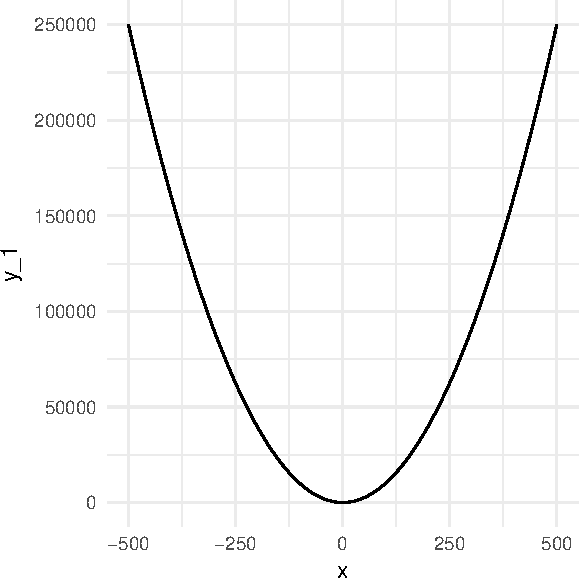
\includegraphics{Optimization_files/figure-latex/FOC_dim_1-1.pdf}

End points or corner points are generally not considered critical points
though they can contain extreme points. (For the plot \(f(x)=x^2\) what
is/are maximal points if \(x\in [l, b]\)?) Conventionally, critical
points are thought to be points interior to the domain.

Functions can be separated into classes on the basis of how
differentiable they are (the differentiability class). For example, all
functions that are continuous form the \(C^0\) class; those that are
differentiable and their derivatives also continuous form the class
\(C^1\); those whose second derivatives are continuous form the class
\(C^2\) and so on.\footnote{A function is ``smooth'' if all derivatives
  are continous: \(f\in C^{\infty}\); and analytical
  \(f \in C^{\omega}\) if it is smooth \emph{and} its Taylor
  approximation converges to its function value at all points in the
  domain.}

\textbf{Theorem:} If \(x^*\in \mathbb{R}^n\) is an interior point in the
domain of the real-valued function \(F\in C^1\), then it is a critical
point when \[
  \frac{\partial F}{\partial x_i}(x^*) = 0, i\in \{1, 2,\hdots, n\}
\]

\subsection{Second Order Conditions}\label{second-order-conditions}

Critical points are interior points at which all first partial
derivatives are 0. However, this in itself is not enough for us to know
if the critical point is a maximum, a minimum or neither. For this, we
need to consider its second derivatives.

For the function \(F\in C^2, x\in U\subset \mathbb{R}^n\), (\(U\) is
open in \(\mathbb{R}^n\)) the \emph{Hessian} is the following second
derivative matrix: \[
D^2F(x^*) = \begin{bmatrix}
\frac{\partial F}{\partial x_1^2}(x^*) & \hdots &\frac{\partial F}{\partial x_n\partial x_1}(x^*)\\
\vdots & \ddots & \vdots\\
\frac{\partial F}{\partial x_1\partial x_n}(x^*) & \hdots & \frac{\partial F}{\partial x_n^2}(x^*)
\end{bmatrix}
\]

The second order conditions are based on the Hessian. Just as in the one
dimensional case, where there occurs a maximum at a critical point if
the second derivative is negative; there occurs a maximum at the
critical point \(x^*\in U\subset \mathbb{R}^n\) if the Hessian is
\emph{negative definite}.


\end{document}
